\documentclass[12pt]{extarticle}
\usepackage[left = 2cm, right = 2cm, top = 2cm, bottom = 2cm]{geometry}
\usepackage{graphicx}
\usepackage{amsmath}
\usepackage{amssymb}
\usepackage{hyperref}
\usepackage{listings}
\usepackage{caption}
\usepackage{subcaption}
\usepackage{multirow}
\usepackage{bm}
\usepackage{float}
\usepackage{placeins}
\usepackage{pdfpages}

\begin{document}

\begin{flushleft}
\begin{LARGE}
\textbf{14.6}
\end{LARGE}  
\end{flushleft}

\vfill
\begin{center}
\begin{Huge}
Isolating Integrals for Geodesic Motion
\end{Huge}
\end{center}
\vfill

\pagebreak

\begin{center}
\textbf{Question 1}
\end{center}

We have the general axisymmetric metric 
$$\mathrm{d}s^2 = g_{tt}\mathrm{d}t^2+2g_{t\phi}\mathrm{d}t \mathrm{d}\phi +g_{\phi \phi} \mathrm{d}\phi ^2+g_{rr}\mathrm{d}r^2+g_{\theta \theta}\mathrm{d}\theta^2$$

where the $g_{i j}$ are functions of $r$ and $\theta$ only. The Lagrangian and geodesic action are given by
$$\mathcal{L} = \sqrt{g_{\alpha \beta}\frac{\mathrm{d}x^\alpha}{\mathrm{d}\lambda}\frac{\mathrm{d}x^\beta}{\mathrm{d}\lambda}} \;\;,\;\; \mathcal{S} = \int \mathcal{L}\, \mathrm{d}\lambda$$

The proper time $\tau$ is given by 
$$\tau (\lambda) = \int_{0}^{\lambda} \sqrt{g_{\alpha \beta}\frac{\mathrm{d}x^\alpha}{\mathrm{d}\tilde{\lambda}}\frac{\mathrm{d}x^\beta}{\mathrm{d}\tilde{\lambda}}} \mathrm{d}\tilde{\lambda}
\; \Rightarrow \; \frac{\mathrm{d}\tau}{\mathrm{d}\lambda} = \mathcal{L}$$

Both $t$ and $\phi$ are ignorable coordinates of the Lagrangian and so give rise to conserved quantities. 

\begin{align*}
\frac{\partial \mathcal{L}}{\partial t}&=\frac{\mathrm{d}}{\mathrm{d}\lambda}\left(\frac{\partial \mathcal{L}}{\partial \dot{t}}\right)  & \frac{\partial \mathcal{L}}{\partial \phi}&=\frac{\mathrm{d}}{\mathrm{d}\lambda}\left(\frac{\partial \mathcal{L}}{\partial \dot{\phi}}\right) \\
0&=\frac{\mathrm{d}}{\mathrm{d}\lambda}\left(\frac{\partial \mathcal{L}}{\partial \dot{t}}\right)& 0&= \frac{\mathrm{d}}{\mathrm{d}\lambda}\left(\frac{\partial \mathcal{L}}{\partial \dot{\phi}}\right) \\
E&=\frac{\partial \mathcal{L}}{\partial \dot{t}} &L_z &= -\frac{\partial \mathcal{L}}{\partial \dot{\phi}}\\
E&=\frac{1}{2\mathcal{L}}\left(2g_{tt}\frac{\mathrm{d}t}{\mathrm{d}\lambda}+2g_{t\phi}\frac{\mathrm{d}\phi}{\mathrm{d}\lambda}\right) &L_z &= -\frac{1}{2\mathcal{L}}\left(2g_{t\phi}\frac{\mathrm{d}t}{\mathrm{d}\lambda}+2g_{\phi\phi}\frac{\mathrm{d}\phi}{\mathrm{d}\lambda}\right)\\
E&= \frac{\mathrm{d}\lambda}{\mathrm{d}\tau}\left(g_{tt}\frac{\mathrm{d}t}{\mathrm{d}\lambda}+g_{t\phi}\frac{\mathrm{d}\phi}{\mathrm{d}\lambda}\right) & L_z &=-\frac{\mathrm{d}\lambda}{\mathrm{d}\tau}\left(g_{t\phi}\frac{\mathrm{d}t}{\mathrm{d}\lambda}+g_{\phi\phi}\frac{\mathrm{d}\phi}{\mathrm{d}\lambda}\right)\\
E &= g_{tt}\frac{\mathrm{d}t}{\mathrm{d}\tau}+g_{t\phi}\frac{\mathrm{d}\phi}{\mathrm{d}\tau} & L_z &= -\left(g_{t\phi}\frac{\mathrm{d}t}{\mathrm{d}\tau}+g_{\phi\phi}\frac{\mathrm{d}\phi}{\mathrm{d}\tau}\right)\\
\end{align*}
So $E$ and $L_z$ are constants of geodesic motion. We rearrange these to obtain
$$\dot{t} = \frac{g_{\phi \phi}E+g_{t\phi}L_z}{g_{tt}g_{\phi \phi}-g_{t\phi}^2} \;\;, \;\; \dot\phi = -\frac{g_{t\phi}E+g_{tt}L_z}{g_{tt}g_{\phi \phi}-g_{t\phi}^2}$$

Here we are considering massive particles which move on timelike geodesics. Since $\mathcal{L}$ has no explicit dependence on $\lambda$ we can set $\mathcal{L} = 1$.
$$g_{tt}\dot{t}^2+2g_{t\phi}\dot{t}\dot{\phi}+g_{\phi \phi}\dot{\phi}^2+g_{rr}\dot{r}^2+g_{\theta \theta}\dot{\theta}^2 = 1$$
$$g_{rr}\dot{r}^2+g_{\theta \theta}\dot{\theta}^2 = 1 -g_{tt}\left(\frac{g_{\phi \phi}E+g_{t\phi}L_z}{g_{tt}g_{\phi \phi}-g_{t\phi}^2}\right)^2+
2g_{t\phi}\left(\frac{g_{\phi \phi}E+g_{t\phi}L_z}{g_{tt}g_{\phi \phi}-g_{t\phi}^2}\right)\left(\frac{g_{t\phi}E+g_{tt}L_z}{g_{tt}g_{\phi \phi}-g_{t\phi}^2}\right)-
g_{\phi \phi}\left(\frac{g_{t\phi}E+g_{tt}L_z}{g_{tt}g_{\phi \phi}-g_{t\phi}^2}\right)^2$$

$$g_{rr}\dot{r}^2+g_{\theta \theta}\dot{\theta}^2 = 1 -\frac{1}{\left(g_{tt}g_{\phi\phi}-g_{t\phi}^2\right)^2}\left(E^2 \left(g_{tt}g_{\phi\phi}^2-g_{t\phi}^2g_{\phi\phi}\right)+2EL_z\left(g_{tt}g_{t\phi}g_{\phi \phi} - g_{t\phi}^3 \right) + L_z^2\left(-g_{tt}g_{t\phi}^2+g_{tt}^2 g_{\phi \phi}\right)\right)$$

$$g_{rr}\dot{r}^2+g_{\theta \theta}\dot{\theta}^2 = 1 - \frac{\left(g_{\phi \phi}E^2+2g_{t\phi}EL_z+g_{tt}L_z^2\right)}{g_{tt}g_{\phi\phi}-g_{t\phi}^2}$$

$$g_{rr}\left(\frac{\mathrm{d}r}{\mathrm{d}\tau}\right)^2+g_{\theta \theta}\left(\frac{\mathrm{d}\theta}{\mathrm{d}\tau}\right)^2 = -V_{\mathrm{eff}}(r,\theta,E,L_z)$$

This is the mass conservation integral. The effective potential $V_{\mathrm{eff}}$ is given by
$$V_{\mathrm{eff}}(r,\theta,E,L_z) = \frac{\left(g_{\phi \phi}E^2+2g_{t\phi}EL_z+g_{tt}L_z^2\right)}{g_{tt}g_{\phi\phi}-g_{t\phi}^2}-1$$

\begin{center}
\textbf{Question 2}
\end{center}

The Kerr metric, used to describe the spacetime around a spinning black hole, has components
$$g_{tt} = 1-\frac{2mr}{\Sigma}, \;\;\; g_{t\phi} = \frac{2amr\sin^2\theta}{\Sigma}, \;\;\; g_{\phi \phi} = -\left(\Delta + \frac{2mr(r^2+a^2)}{\Sigma}\right)\sin^2\theta, \;\;\; g_{rr}-\frac{\Sigma}{\Delta},\;\;\; g_{\theta \theta} = -\Sigma$$ 

Where $\Sigma = r^2+a^2\cos^2\theta,\, \Delta = r^2-2mr+a^2$ and $m$ and $a$ are respectively the mass and spin parameter of the black hole.\\

The Christoffel symbols were derived using Mathematica (figure 1). 

\begin{center}
\textbf{Programming Task}
\end{center}

The four second order timelike geodesic equations 

$$\frac{\mathrm{d}^2x^i}{\mathrm{d}\tau^2} = -\Gamma_{jk}^i\frac{\mathrm{d}x^j}{\mathrm{d}\tau}\frac{\mathrm{d}x^k}{\mathrm{d}\tau}$$

are transformed into eight coupled first order equations by introducing the velocity vector $v^i$.
$$\frac{\mathrm{d}x^i}{\mathrm{d}\tau} = v^i\;,\;\frac{\mathrm{d}v^i}{\mathrm{d}\tau} = -\Gamma_{jk}^iv^jv^k$$

The function NDSolve on Mathematica is used to solve these equations numerically.

\begin{center}
\textbf{Question 3}
\end{center}

We obtain the Schwarzschild metric by setting $a=0$ in the Kerr metric. This corresponds to spacetime around a non-spinning black hole. 
$$\mathrm{d}s^2 = \left(1-\frac{2m}{r}\right)\mathrm{d}t^2-r^2\sin^2\theta \,\mathrm{d}\phi^2-\left(1-\frac{2m}{r}\right)^{-1}\mathrm{d}r^2-r^2\mathrm{d}\theta^2$$

The non-zero Christoffel symbols (figure 2) are
$$\Gamma_{13}^1 = \frac{m}{r(r-2m)},\;\; \Gamma_{23}^2 =\frac{1}{r} ,\;\; \Gamma_{24}^2 = \cot\theta ,\;\; \Gamma_{11}^3 = \frac{m(r-2m)}{r^3} ,\;\; \Gamma_{22}^3 = (2m-r)\sin^2\theta$$
$$ \Gamma_{33}^3 = \frac{m}{2mr-r^2},\;\; \Gamma_{44}^3 =2m-r ,\;\; \Gamma_{22}^4 = -\cos\theta\sin\theta,\;\; \Gamma_{34}^4 =\frac{1}{r}$$

Taking $m=1$ and $\theta = \pi/2$, the effective potential (figure 3) becomes

$$V_{\mathrm{eff}} = \frac{\left(r^2E^2
-\left(1-\frac{2}{r}\right)L_z^2\right)}{r^2\left(1-\frac{2}{r}\right)}-1$$

For bound orbits we need $V_{\mathrm{eff}} \geq 0$. We find that for the case $E = 0.97$, $L=4$ the allowed range of radii is $7.61 \leq r \leq 23.2$. It is worth noting that $r = 3.07$ is also a solution but for values less than this the particle would simply fall into the black hole.\\

\textbf{Part a}\\

Here we consider the initial conditions $r = 15$, $\theta = \pi/2$ and $\mathrm{d}r/\mathrm{d}\tau = 0$. We are free to choose $t = 0$ and $\phi = 0$ initially by the symmetries induced by these coordinates. The other initial conditions are determined using the three conservation laws. \\

The coordinates of the particle were plotted over several orbits (figure 4). There are oscillations both in its radius (between 15.0 and 16.2) and in its angle $\theta$. It is completing whole revolutions with respect to the angle $\phi$ at a constant rate. \\

The errors in the conservation laws were calculated at each point and plotted (figure 5). The errors are of orders $10^{-10}$, $10^{-5}$ and $10^{-7}$ for $E$, $L_z$ and $V_{\mathrm{eff}}$ respectively. Hence we can conclude that the conservation laws are indeed satisfied at a reasonable level of numerical accuracy. \\

\textbf{Part b}\\ 

The above was repeated with the initial radii $r_0 = 8,11,14,17,20,23$. The values of $r$ and $\mathrm{d} r/\mathrm{d} \tau$ were found every time an orbit crossed the equatorial plane, with $\mathrm{d} \theta /\mathrm{d}\tau > 0$ (Table 1). The Poincar\'e maps were plotted for each case (figure 6).\\

In the plots (a) - (d) it is clearly visible the points trace out closed curves. This also seems to hold for plots (e) - (f) but the concentration of points to the right slightly conceals this. This  indicates the possible existence of an extra isolating integral for the motion. \\

\textbf{Part c}\\ 

We now experiment with changing the values of initial $r$, initial $\mathrm{d} r/\mathrm{d} \tau$, $E$ and $L_z$, each in turn.

\begin{itemize}
\item[$-$]\textit{Varying initial $r$} (figure 7). The oscillations in $r$ are greater for more extremal values of $r_0$, since their potentials are further away from the maximum. All rotate in the same $\phi$ direction. 

\item[$-$]\textit{Varying initial $\mathrm{d} r/\mathrm{d} \tau$} (figure 8). The yellow particle ($\dot{r} = -0.08$) begins its motion towards the black hole, as expected. Interestingly, the green particle ($\dot{r} = 0.16$) has been given too much radial velocity and rebounds back into the black hole. 

\item[$-$] \textit{Varying $E$} (figure 9). Increasing the energy $E$ increases the sizes of the oscillations in $r$. Further, the angle $\phi$ increases more slowly; the particles rotate with greater radii yet with the same angular momentum in the z-direction ($L_z$). The period of oscillations of $\theta$ increases.

\item[$-$] \textit{Varying $L_z$} (figure 10). The radial trajectories for all three particles are the same. Decreasing $L_z$ simply realigns more angular momentum with the perpendicular plane. This explains the greater variations in the angle $\theta$; it contributes more angular momentum to the total.\\

\end{itemize}

\begin{center}
\textbf{Question 4}
\end{center}

We now consider motion in the Kerr metric and take $a = 0.9$, $E = 0.95$ and $L_z = 3$. Using the effective potential, we find the allowed range of $r_0$ for which the initial conditions $\theta = \pi/2$ and $\mathrm{d}r/\mathrm{d}\tau = 0$ lead to bound motion is $4.51 \leq r \leq 14.6$.\\

The trajectories of particles (figure 11) are similar to those exhibited in the Schwarzschild metric. There are more rapid oscillations in the variables $r$, $\phi$ and $\theta$ due to the spin of the black hole. \\

The Poincar\'e maps (figure 12) take a similar shape to those displayed by the Schwarzschild metric. This indicates the possibility of an additional conserved quantity in the Kerr metric.\\

\begin{center}
\textbf{Question 5}
\end{center}

We have the quantity 
$$Q = (aE\sin\theta - L_z \mathrm{cosec}\theta)^2+(r^2+a^2\cos^2\theta)^2\left(\frac{\mathrm{d}\theta}{\mathrm{d}\tau}\right)^2+\delta a^2 \cos^2\theta$$

We use Mathematica to show it is conserved (figure 13). We apply the chain rule and substitute for $\dot{r}$, $E$, $L_z$ and $\ddot{\theta}$ using the conservation laws and the $\ddot{\theta}$ geodesic equation. The final result is 
$$\frac{\mathrm{d}Q}{\mathrm{d}\tau} = a^2(1-\delta)\dot{\theta}\sin2\theta$$
  
For $Q$ to be conserved we need $\delta = 1$. In the Schwarzschild metric (the limit $a=0$), $Q$ becomes
\begin{align*}
Q &= L_z^2 \mathrm{cosec}^2\theta+r^4\left(\frac{\mathrm{d}\theta}{\mathrm{d}\tau}\right)^2 \\
Q &= \left(-g_{t\phi}\frac{\mathrm{d}t}{\mathrm{d}\tau}-g_{\phi \phi}\frac{\mathrm{d}\phi}{\mathrm{d}\tau}\right)^2\mathrm{cosec}^2\theta+r^4\left(\frac{\mathrm{d}\theta}{\mathrm{d}\tau}\right)^2\\
Q &= \left(r^2\sin^2\theta\frac{\mathrm{d}\phi}{\mathrm{d}\tau}\right)^2\mathrm{cosec}^2\theta+r^4\left(\frac{\mathrm{d}\theta}{\mathrm{d}\tau}\right)^2\\
Q &= r^4\left( \sin^2\theta \left(\frac{\mathrm{d}\phi}{\mathrm{d}\tau}\right)^2+\left(\frac{\mathrm{d}\theta}{\mathrm{d}\tau}\right)^2\right)
\end{align*}

In spherical polars, the angular momentum vector is given by

$$\textbf{L} = m\textbf{r}\times\textbf{v} = mr^2(\dot{\theta}\bm{\hat{\phi}}-\dot{\phi}\sin\theta \bm{\hat{\theta})}$$

So $Q$ is exactly the square of the total angular momentum. We find that the total angular momentum is conserved. This is probably not exactly true in the Kerr metric due to the spin of the black hole. 

\pagebreak
\begin{center}
\textbf{Figures and tables}
\end{center}

\begin{figure}[bh!]
    \centering
    \begin{subfigure}[b]{0.85\textwidth}
        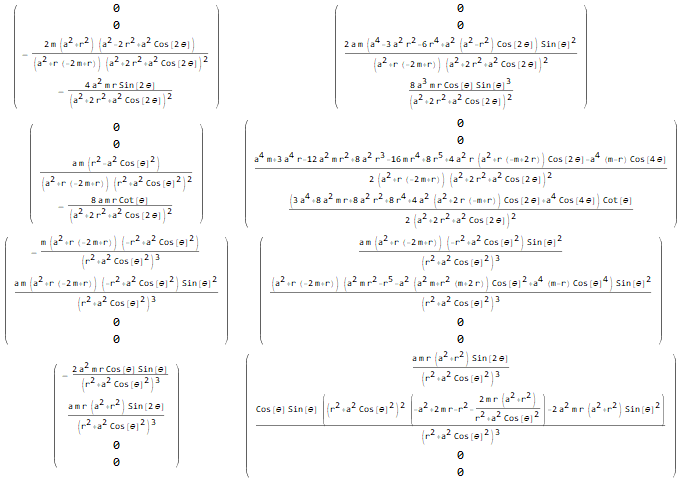
\includegraphics[width=\textwidth]{Christoffel_Kerr_1.png}
        \caption{Columns 1 and 2}
        \label{figure:1a}
    \end{subfigure}  
    \\
    \begin{subfigure}[b]{0.85\textwidth}
        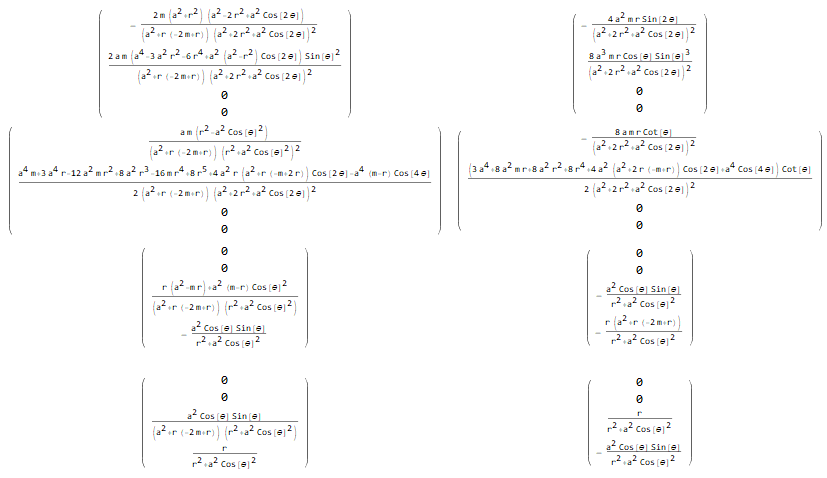
\includegraphics[width=\textwidth]{Christoffel_Kerr_2.png}
        \caption{Columns 3 and 4}
        \label{figure:1b}
    \end{subfigure} 
    \caption{The Christoffel symbols for the Kerr metric. Each row corresponds to a value of $i$, each column to a value of $j$ and each sub-row to a value of $k$.}
    \label{figure 1}
\end{figure}

\begin{figure}[h]
\centering
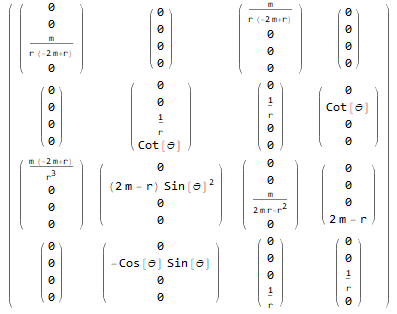
\includegraphics[scale=1]{Christoffel_Sch.png}\\
\caption{Christoffel symbols for the Schwarzschild metric}
\label{figure:2}
\end{figure}

\begin{figure}[h]
\centering
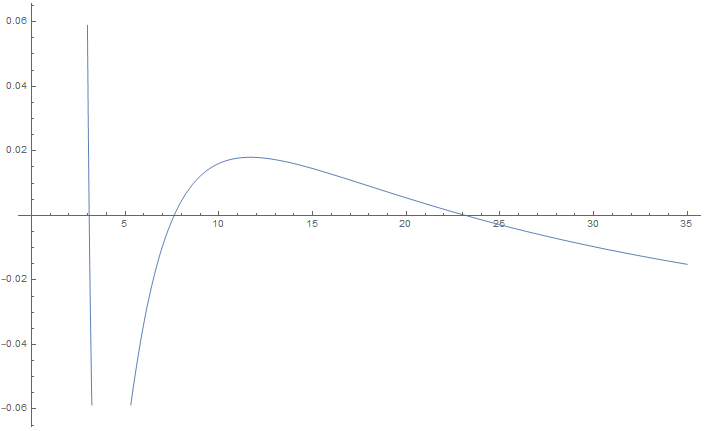
\includegraphics[scale=0.6]{PotentialSch.png}\\
\caption{Plot of the effective potential}
\label{figure:3}
\end{figure}

\begin{figure}[h]
    \centering
    \begin{subfigure}[b]{0.4\textwidth}
        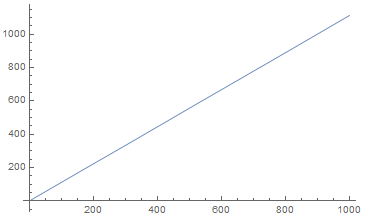
\includegraphics[width=\textwidth]{parta_t.png}
        \caption{Plot of $t(\tau)$}
        \label{figure:4a}
    \end{subfigure}  
    \qquad
    \begin{subfigure}[b]{0.4\textwidth}
        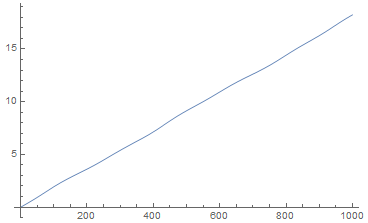
\includegraphics[width=\textwidth]{parta_phi.png}
        \caption{Plot of $\phi(\tau)$}
        \label{figure:4b}
    \end{subfigure} 
    \\ 
    \begin{subfigure}[b]{0.4\textwidth}
        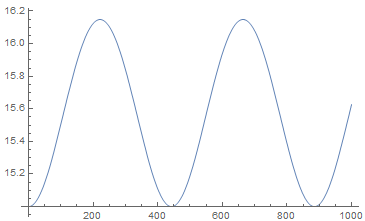
\includegraphics[width=\textwidth]{parta_r.png}
        \caption{Plot of $r(\tau)$}
        \label{figure:4c}
    \end{subfigure} 
    \qquad
    \begin{subfigure}[b]{0.4\textwidth}
        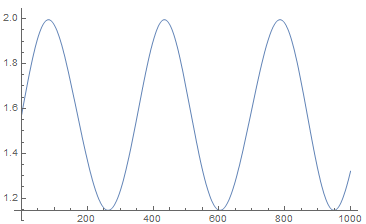
\includegraphics[width=\textwidth]{parta_theta.png}
        \caption{Plot of $\theta(\tau)$}
        \label{figure:4d}
    \end{subfigure}
    \caption{Plots of the coordinates of the particle over several orbits}\label{figure 4}
\end{figure}

\begin{figure}[h]
    \centering
    \begin{subfigure}[b]{0.45\textwidth}
        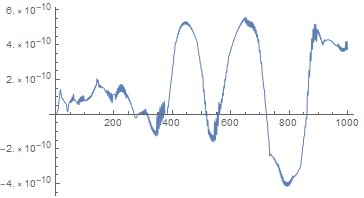
\includegraphics[width=\textwidth]{numeracc_E.png}
        \caption{Error in $E$}
        \label{figure:5a}
    \end{subfigure}  
    \qquad
    \begin{subfigure}[b]{0.45\textwidth}
        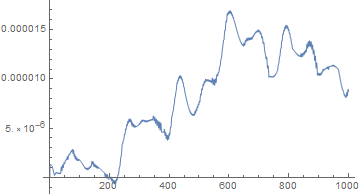
\includegraphics[width=\textwidth]{numeracc_Lz.png}
        \caption{Error in $L_z$}
        \label{figure:5b}
    \end{subfigure} 
    \qquad
    \begin{subfigure}[b]{0.45\textwidth}
        \includegraphics[width=\textwidth]{numeracc_v.png}
        \caption{Error in $V_{\mathrm{eff}}$}
        \label{figure:5c}
    \end{subfigure}
    \caption{Numerical Errors in the three conservation laws} 
    \label{figure 5}
\end{figure}

\begin{figure}[h]
    \centering
    \begin{subfigure}[b]{0.4\textwidth}
        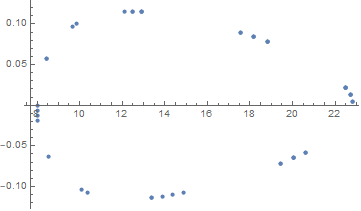
\includegraphics[width=\textwidth]{3b_r_8.png}
        \caption{$r_0 = 8 $}
        \label{figure:6a}
    \end{subfigure}  
    \qquad
    \begin{subfigure}[b]{0.4\textwidth}
        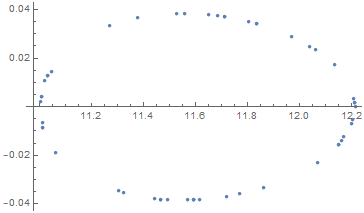
\includegraphics[width=\textwidth]{3b_r_11.png}
        \caption{$r_0 = 11 $}
        \label{figure:6b}
    \end{subfigure} 
    \\
    \begin{subfigure}[b]{0.4\textwidth}
        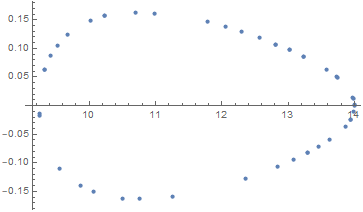
\includegraphics[width=\textwidth]{3b_r_14.png}
        \caption{$r_0 = 14 $}
        \label{figure:6c}
    \end{subfigure}
    \qquad
    \begin{subfigure}[b]{0.4\textwidth}
        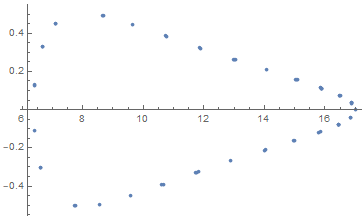
\includegraphics[width=\textwidth]{3b_r_17.png}
        \caption{$r_0 = 17 $}
        \label{figure:6d}
    \end{subfigure}  
    \\
    \begin{subfigure}[b]{0.4\textwidth}
        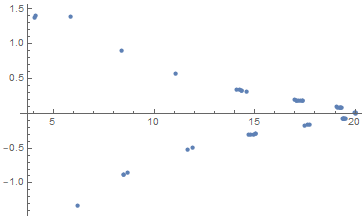
\includegraphics[width=\textwidth]{3b_r_20.png}
        \caption{$r_0 =20 $}
        \label{figure:6e}
    \end{subfigure} 
    \qquad
    \begin{subfigure}[b]{0.4\textwidth}
        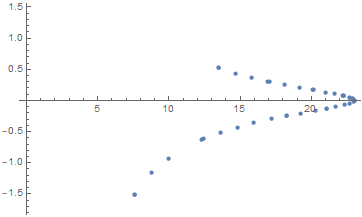
\includegraphics[width=\textwidth]{3b_r_23.png}
        \caption{$r_0 = 23 $}
        \label{figure:6f}
    \end{subfigure} 
    \caption{Poincar\'e maps of the orbits} 
    \label{figure 6}
\end{figure}

\begin{figure}[h]
    \centering
    \begin{subfigure}[b]{0.4\textwidth}
        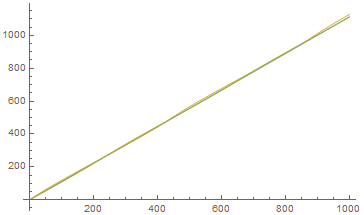
\includegraphics[width=\textwidth]{3c_ra_t.png}
        \caption{Plot of $t$}
        \label{figure:7a}
    \end{subfigure}  
    \qquad
    \begin{subfigure}[b]{0.4\textwidth}
        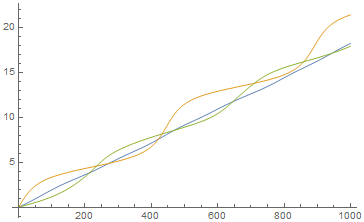
\includegraphics[width=\textwidth]{3c_ra_phi.png}
        \caption{Plot of $\phi$}
        \label{figure:7b}
    \end{subfigure} 
    \\ 
    \begin{subfigure}[b]{0.4\textwidth}
        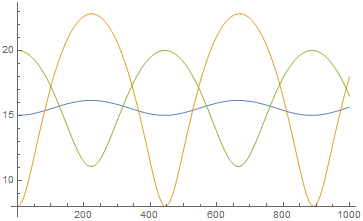
\includegraphics[width=\textwidth]{3c_ra_r.png}
        \caption{Plot of $r$}
        \label{figure:7c}
    \end{subfigure} 
    \qquad
    \begin{subfigure}[b]{0.4\textwidth}
        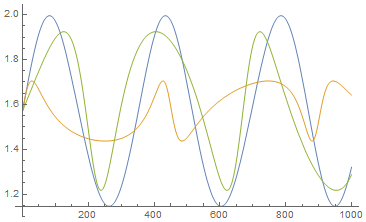
\includegraphics[width=\textwidth]{3c_ra_theta.png}
        \caption{Plot of $\theta$}
        \label{figure:7d}
    \end{subfigure}
    \caption{Plots with initial $r$ varying. The values 8, 15 and 20 in yellow, blue and green.}
    \label{figure 7}
\end{figure}

\begin{figure}[h]
    \centering
    \begin{subfigure}[b]{0.4\textwidth}
        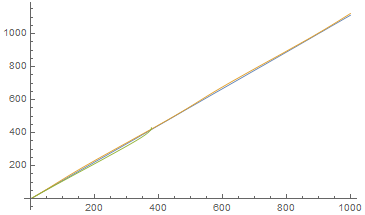
\includegraphics[width=\textwidth]{3c_R_t.png}
        \caption{Plot of $t$}
        \label{figure:8a}
    \end{subfigure}  
    \qquad
    \begin{subfigure}[b]{0.4\textwidth}
        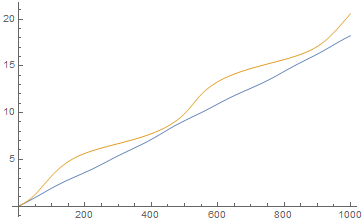
\includegraphics[width=\textwidth]{3c_R_phi.png}
        \caption{Plot of $\phi$}
        \label{figure:8b}
    \end{subfigure} 
    \\ 
    \begin{subfigure}[b]{0.4\textwidth}
        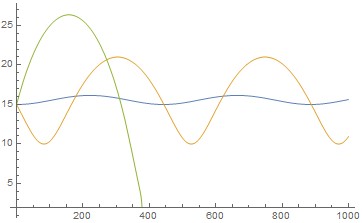
\includegraphics[width=\textwidth]{3c_R_r.png}
        \caption{Plot of $r$}
        \label{figure:8c}
    \end{subfigure} 
    \qquad
    \begin{subfigure}[b]{0.4\textwidth}
        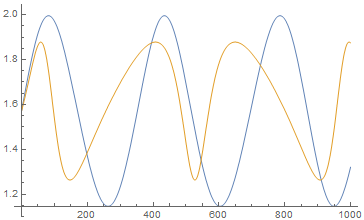
\includegraphics[width=\textwidth]{3c_R_theta.png}
        \caption{Plot of $\theta$}
        \label{figure:8d}
    \end{subfigure}
    \caption{Plots with initial $\mathrm{d}r/\mathrm{d}\tau$ varying. The values -0.08, 0 and 0.16 in yellow, blue and green.}
    \label{figure 8}
\end{figure}

\begin{figure}[h]
    \centering
    \begin{subfigure}[b]{0.4\textwidth}
        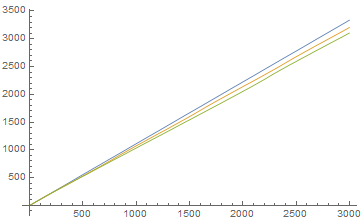
\includegraphics[width=\textwidth]{3c_E_t.png}
        \caption{Plot of $t$}
        \label{figure:9a}
    \end{subfigure}  
    \qquad
    \begin{subfigure}[b]{0.4\textwidth}
        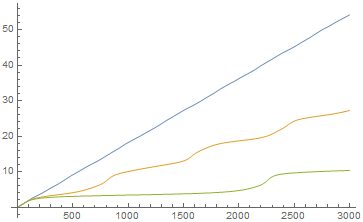
\includegraphics[width=\textwidth]{3c_E_phi.png}
        \caption{Plot of $\phi$}
        \label{figure:9b}
    \end{subfigure} 
    \\ 
    \begin{subfigure}[b]{0.4\textwidth}
        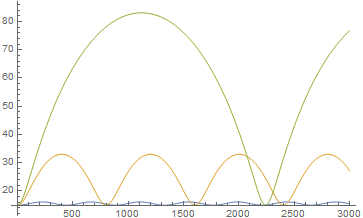
\includegraphics[width=\textwidth]{3c_E_r.png}
        \caption{Plot of $r$}
        \label{figure:9c}
    \end{subfigure} 
    \qquad
    \begin{subfigure}[b]{0.4\textwidth}
        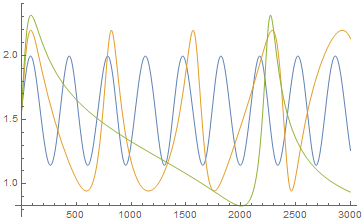
\includegraphics[width=\textwidth]{3c_E_theta.png}
        \caption{Plot of $\theta$}
        \label{figure:9d}
    \end{subfigure}
    \caption{Plots with initial $E$ varying. The values 0.97, 0.98 and 0.99 in blue, yellow and green.}
    \label{figure 9}
\end{figure}

\begin{figure}[h]
    \centering
    \begin{subfigure}[b]{0.4\textwidth}
        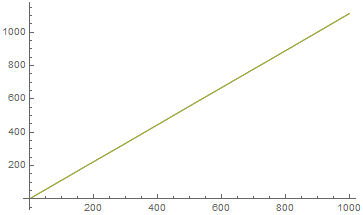
\includegraphics[width=\textwidth]{3c_Lz_t.png}
        \caption{Plot of $t$}
        \label{figure:10a}
    \end{subfigure}  
    \qquad
    \begin{subfigure}[b]{0.4\textwidth}
        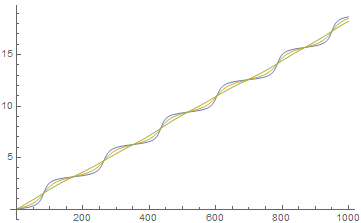
\includegraphics[width=\textwidth]{3c_Lz_phi.png}
        \caption{Plot of $\phi$}
        \label{figure:10b}
    \end{subfigure} 
    \\ 
    \begin{subfigure}[b]{0.4\textwidth}
        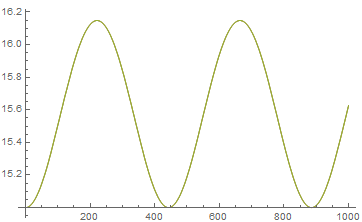
\includegraphics[width=\textwidth]{3c_Lz_r.png}
        \caption{Plot of $r$}
        \label{figure:10c}
    \end{subfigure} 
    \qquad
    \begin{subfigure}[b]{0.4\textwidth}
        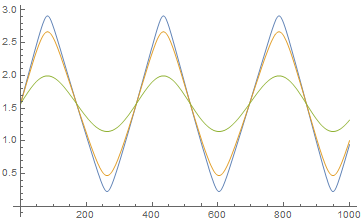
\includegraphics[width=\textwidth]{3c_Lz_theta.png}
        \caption{Plot of $\theta$}
        \label{figure:10d}
    \end{subfigure}
    \caption{Plots with initial $L_z$ varying. The values 1, 2 and 4 in blue, yellow and green.}
    \label{figure 10}
\end{figure}

\begin{figure}[h]
    \centering
    \begin{subfigure}[b]{0.4\textwidth}
        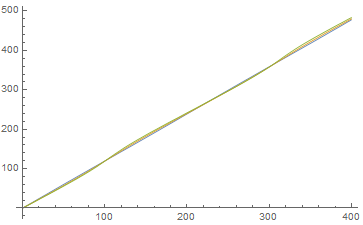
\includegraphics[width=\textwidth]{4_t.png}
        \caption{Plot of $t$}
        \label{figure:11a}
    \end{subfigure}  
    \qquad
    \begin{subfigure}[b]{0.4\textwidth}
        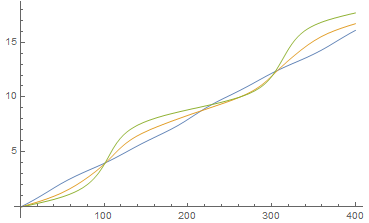
\includegraphics[width=\textwidth]{4_phi.png}
        \caption{Plot of $\phi$}
        \label{figure:11b}
    \end{subfigure} 
    \\ 
    \begin{subfigure}[b]{0.4\textwidth}
        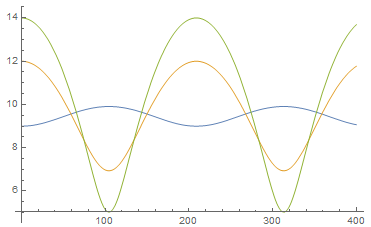
\includegraphics[width=\textwidth]{4_r.png}
        \caption{Plot of $r$}
        \label{figure:11c}
    \end{subfigure} 
    \qquad
    \begin{subfigure}[b]{0.4\textwidth}
        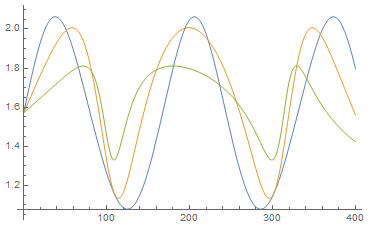
\includegraphics[width=\textwidth]{4_theta.png}
        \caption{Plot of $\theta$}
        \label{figure:11d}
    \end{subfigure}
    \caption{Plots with initial $r$ varying. The values 9,12 and 14 in blue, yellow and green.}
    \label{figure 11}
\end{figure}

\begin{figure}[h]
    \centering
    \begin{subfigure}[b]{0.4\textwidth}
        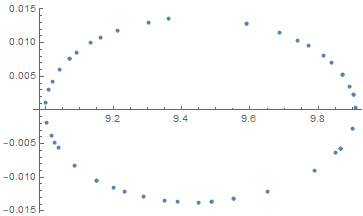
\includegraphics[width=\textwidth]{4_poincare_9.png}
        \caption{$r_0 = 9 $}
        \label{figure:12a}
    \end{subfigure}  
    \qquad
    \begin{subfigure}[b]{0.4\textwidth}
        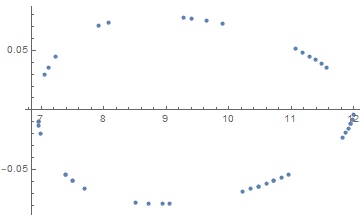
\includegraphics[width=\textwidth]{4_poincare_12.png}
        \caption{$r_0 = 12 $}
        \label{figure:12b}
    \end{subfigure} 
    \qquad
    \begin{subfigure}[b]{0.4\textwidth}
        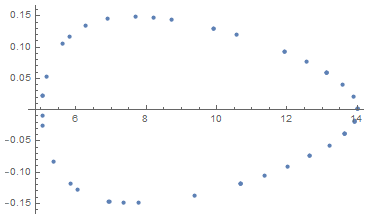
\includegraphics[width=\textwidth]{4_poincare_14.png}
        \caption{$r_0 = 14 $}
        \label{figure:12c}
    \end{subfigure}
    \caption{Poincar\'e maps of the orbits} 
    \label{figure 12}
\end{figure}

\FloatBarrier

\begin{figure}[h]
\centering
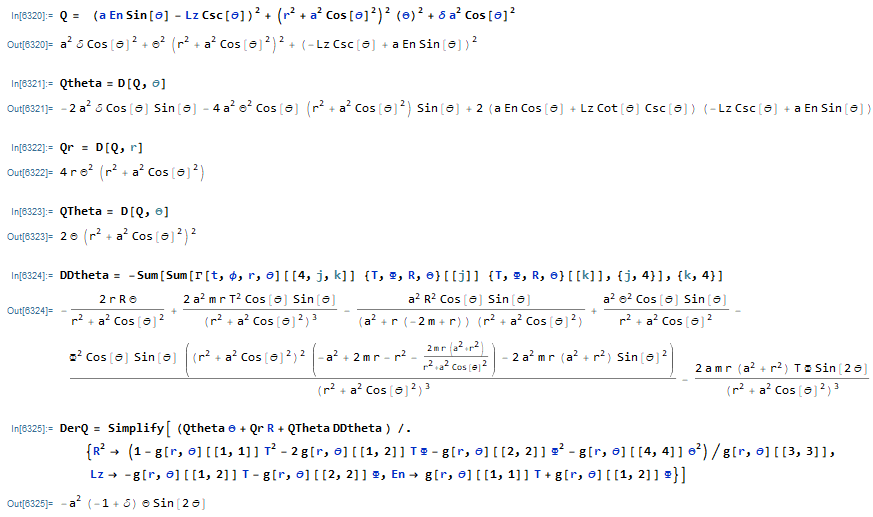
\includegraphics[scale=0.78]{Q5.png}\\
\caption{Calculation of $\frac{\mathrm{d}Q}{\mathrm{
d}\tau}$}
\label{figure:13}
\end{figure}

\begin{table}[!htbp]
\centering
\begin{tabular}{|c||ccccccc|}
\hline
\multirow{2}{2em}{$r_0$} & \multicolumn{7}{c|}{Values of $r$}\\ 
& \multicolumn{7}{c|}{Values of $\mathrm{d} r/\mathrm{d} \tau$}\\
\hline \hline
\multirow{2}{2em}{8.00}& 18.8 & 13.4 & 18.8 & $\hdots$ & 12.1&14.9 &8.04  \\ 
 & 0.078&-0.114 &0.078 & $\hdots$ & 0.115&-0.108 &  -0.0183\\ 
\hline
\multirow{2}{2em}{11.0}& 11.8 & 12.2 & 12.2 & $\hdots$ & 11.3& 11.6& 12.1 \\ 
& -0.0358 & -0.0124& 0.00354 & $\hdots$ & -0.0345 & -0.0382& -0.0231 \\ 
\hline
\multirow{2}{2em}{14.0} & 12.1 & 11.0 & 9.24 & $\hdots$ & 14.0 & 13.6 & 10.7 \\ 
& 0.138&0.162 &-0.0138 & $\hdots$ & 0.014&0.0625 & 0.163 \\ 
\hline
\multirow{2}{2em}{17.0} & 15.0 & 13.0 & 7.11 & $\hdots$ & 16.9 & 15.8 & 16.8 \\ 
& 0.16 & 0.264 & 0.449 & $\hdots$ & 0.0334 & -0.119 & -0.0401 \\ 
\hline
\multirow{2}{2em}{20.0} & 17.4 & 17.4 & 14.6 & $\hdots$ & 19.1 &17.0 &14.1  \\ 
& 0.178&0.178 &0.317 & $\hdots$ &0.0939 & 0.196 & 0.344 \\ 
\hline
\multirow{2}{2em}{23.0} & 22.3 & 20.2 & 17.1 & $\hdots$ & 16.9 &8.81 &12.5  \\ 
& 0.076 & 0.168 & 0.300 &$\hdots$ & 0.307 &-1.16 & -0.614  \\ 
\hline
\end{tabular}
\caption{Data for the Poincar\'e maps}
\label{Table:1}
\end{table}

\begin{center}
\textbf{End of Project}
\end{center}
\pagebreak

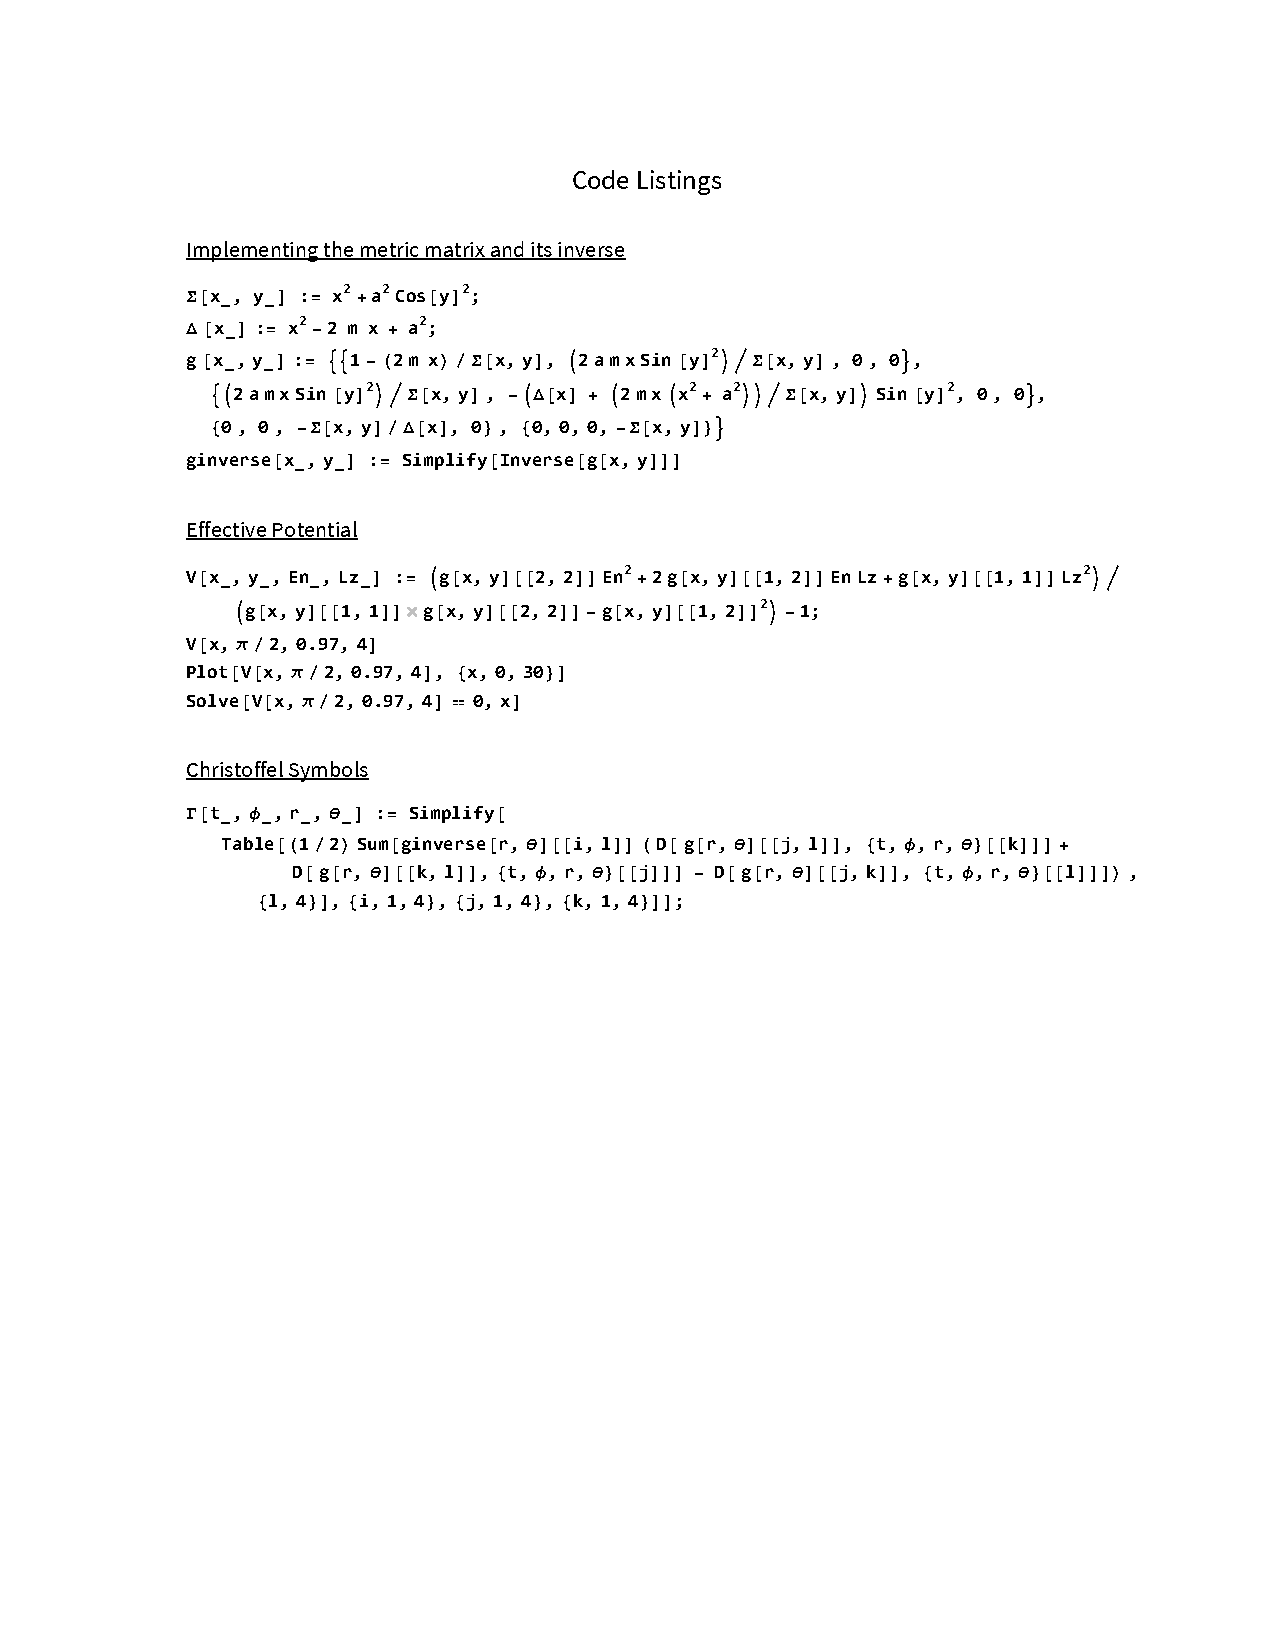
\includepdf[pages=-]{code.pdf}

\end{document}
